\section{\scshape Model}

\subsection{Opis modelu}
\begin{frame}{Opis modelu}
	\begin{itemize}
	\item Dane o propagacji dymu generowane przez FDS
	\item Symulacja dyskretna
	\item Automat komórkowy wykorzystujący sąsiedztwo Moore'a
	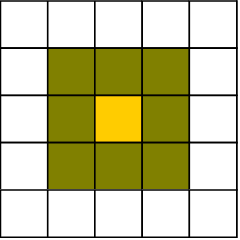
\includegraphics[keepaspectratio=true, scale=0.75]{moore}
	\item Dynamiczne i statyczne pola potencjału
	\item Wykorzystanie proksemiki
	\end{itemize}
\end{frame}

\subsection{Teoria proksemiki}
\begin{frame}{Teoria proksemiki}
\end{frame}

\subsection{Reprezentacja ewakuowanego}
\begin{frame}{Reprezentacja ewakuowanego}
\end{frame}

\subsection{Funkcja kosztu}
\begin{frame}{Funkcja kosztu}
\end{frame}